\chapter{Linear programming}
\label{cha:introduction-1}

We start by giving some examples of linear programs and how they are
used in practice. 
 





\section{Softdrink production}
\label{sec:healthy-low-priced}

Imagine that you own a company that produces the two softdrinks,
\emph{Spring} and \emph{Nebsi}. These softdrinks are a mixture of
\emph{water}, an ingredient \emph{A} and ingredient \emph{B}.
The recipes for Spring and Nebsi are different. Also, the profit for the two drinks is not the same. Those are as follows. 

The use  of ingredients A and B and the profit  per $100l$ are as follows. 
\begin{center}
  \begin{tabular}{c|c|c|c}
    &  A &  B & Profit  \\\hline
    Spring      & $3l$          & $8l$ & $100$ CHF\\\hline 
    Nebsi      & $6l$           & $4l$ & $125$ CHF
  \end{tabular}
\end{center}
%
While the supply of water is unlimited, your company has only $30l$ of
ingredient~$A$ and $44l$ of ingredient~$B$.

At the end of the production day, the local wholesaler picks up the
drinks in two barrels. The capacity of the barrel for Spring is $500l$
while the barrel for Nebsi has a capacity of $400l$.

As the manager of your small company, your goal is to come up with a
\emph{production plan} that maximizes your profit. A production plan
is a two-dimensional vector $(x_1,x_2) \in \R^2$ which means that you
will produce $x_1 \cdot 100 l$ of Spring and $x_2 \cdot 100 l$ of
Nebsi. A production plan is \emph{feasible} if the produced drinks fit
into the respective barrels and not more of A and B is used than what
is on stock. Clearly, $(5,4)$ is not a feasible production plan, as
this would require $39l$ of ingredient A which exceeds the capacity.





A feasible production plan that maximizes your profit can be found
with the help of a \emph{linear program}, a central object of study in
this course.

  \begin{equation}\label{eq:1-4}
  \begin{array}[]{l rcl}
    \text{max.} & 100\cdot x_1 + 125 \cdot x_2 \\
    \text{ s.t.:} &  3\cdot x_1 + 6 \cdot x_2 & \leq & 30 \\
    &    8\cdot x_1 + 4 \cdot x_2 & \leq & 44 \\
    & x_1 & \leq & 5\\
    & x_2 & \leq & 4\\
     & x_1 & \geq & 0\\
    & x_2 & \geq & 0\\
  \end{array}
\end{equation}

One has to maximize a linear \emph{objective function}, in this case
$f(x_1,x_2) = 100\cdot x_1 + 125 \cdot x_2$ where $(x_1,x_2)$
satisfies linear inequalities. The linear inequalities $x_1\geq 0$ and
$x_2 \geq 0$ reflect the fact that only positive amounts can be
produced, while $x_1 \leq 5$ reflects the barrel capacity for
Spring. The linear inequality $3\cdot x_1 + 6 \cdot x_2 \leq 30$
reflects the amount of $30l$ of ingredient A that is on stock.

We can now make a drawing of all feasible production plans. 


\begin{figure}
  \centering
  
  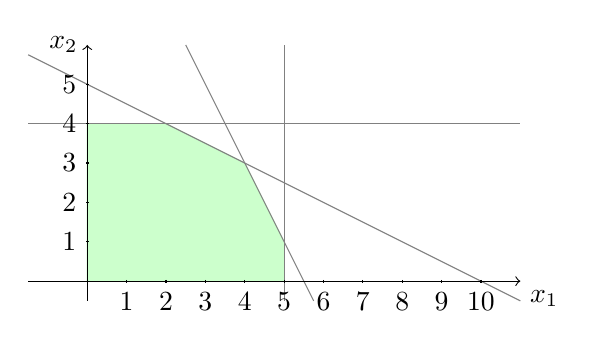
\begin{tikzpicture}[scale=.5]       
     
          \filldraw[fill=green!20,draw=green!20!](0,0) -- (0,4) -- (2,4) --
          (4,3) -- (5,1) -- (5,0) -- (0,0); 
     
          
          \draw [-,draw=gray] (11,-.5) -- (-1.5,5.75) ;
          \draw [-,draw=gray] (-1.5,4) -- (11,4) ;
          \draw [-,draw=gray] (5,-.5) -- (5,6) ;
          \draw [-,draw=gray] (2.5,6) -- (5.75,-.5) ;
                              
          
          
          \draw[->] (-1.5,0) -- (11,0) node[below right] {$x_1$}; \draw[->]
          (0,-.5) -- (0,6) node[left] {$x_2$};
          
          
          \foreach \x in {1,...,10}
          \draw (\x cm,1pt) -- (\x cm,-1pt) node[anchor=north] {$\x$};
          \foreach \y in {1,...,5}
          \draw (1pt,\y cm) -- (-1pt,\y cm) node[anchor=east] {$\y$};     
        \end{tikzpicture} 

  \caption{The feasible production plans are the green area. }
  \label{fig:2}
\end{figure}

The set of points $(x_1,x_2)$ that have objective function $\beta$ is the line 
\begin{displaymath}
  \{(x_1,x_2) \in \R^2 \colon 100\cdot x_1 + 125 \cdot x_2 = \beta \} 
\end{displaymath}
and our task is now to find the largest value for $\beta$ such that the corresponding line still intersects the set of feasible production plans. 


\begin{figure}
  \centering
  
  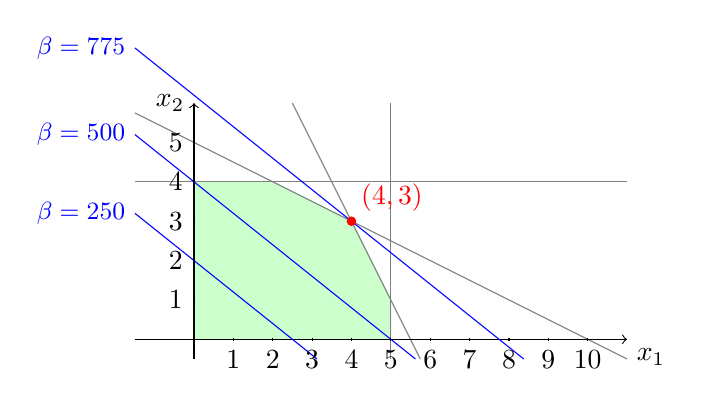
\begin{tikzpicture}[scale=.5]       
     
          \filldraw[fill=green!20,draw=green!20!](0,0) -- (0,4) -- (2,4) --
          (4,3) -- (5,1) -- (5,0) -- (0,0); 
     
          
          \draw [-,draw=gray] (11,-.5) -- (-1.5,5.75) ;
          \draw [-,draw=gray] (-1.5,4) -- (11,4) ;
          \draw [-,draw=gray] (5,-.5) -- (5,6) ;
          \draw [-,draw=gray] (2.5,6) -- (5.75,-.5) ;
                              
          
          
          \draw[->] (-1.5,0) -- (11,0) node[below right] {$x_1$}; \draw[->]
          (0,-.5) -- (0,6) node[left] {$x_2$};
          
          {
          \draw[draw=blue] (-1.50000000000000,
          7.40000000000000)node[left]{\small  
            \color{blue}{$  \beta = 775$}} --
          (8.37500000000000, -0.500000000000000) ; }
 
          {
          \draw[draw = blue] 
          (-1.50000000000000, 5.20000000000000)node[left]{\small 
            \color{blue}{$  \beta = 500$}}
          --
          (5.62500000000000, -0.500000000000000) ; %beta = 500 
}

    
          {      
          \draw[draw = blue] 
          (-1.50000000000000, 3.20000000000000)node[left]{\small 
            \color{blue}{$  \beta = 250$}}
          -- (3.12500000000000, -0.500000000000000); % beta = 250 

        }
         
        {
        \filldraw [red] (4,3) circle (3pt)node[above right] {$(4,3)$};
}
          
          \foreach \x in {1,...,10}
          \draw (\x cm,1pt) -- (\x cm,-1pt) node[anchor=north] {$\x$};
          \foreach \y in {1,...,5}
          \draw (1pt,\y cm) -- (-1pt,\y cm) node[anchor=east] {$\y$};     
        \end{tikzpicture} 

  \caption{The optimal production plan is $(4,3)$.}
  \label{fig:intro3}
\end{figure}
Figure~\ref{fig:intro3} reveals that $(4,3)$ is an optimal production plan and that the maximum profit that the manager can achieve is $775$. 



\section{Proving optimality}
\label{sec:proving-optimality}


How can the manager be convinced that $(4,3)$ is an optimal production
plan? Maybe he has made a mistake in his drawing or with his
calculations and $(4,3)$ is not optimal. What we will see now is a
very important principle of linear programming. There is a simple way
to prove optimality of solutions that we will explore later on. 

Inspecting the drawing, one can see that there are two inequalities that $(4,3)$ satisfies with equality, namely the inequalities 
\begin{eqnarray}
\label{eq:1-2}
    3\cdot x_1 + 6 \cdot x_2 & \leq & 30 \\
     8\cdot x_1 + 4 \cdot x_2 & \leq & 44.  \label{eq:1-3}
\end{eqnarray}
Clearly all feasible production plans satisfy these inequalities and
inspecting Figure~\ref{fig:intro3} it seems clear that $(4,3)$ is an
optimal solution of the optimization problem~\eqref{eq:1-4} where each
linear inequality but the inequalities~\eqref{eq:1-2} and
\eqref{eq:1-3} have been removed. 

What now follows is a very important technique that we will apply later on again in greater generality. Since each feasible production plan satisfies the inequalities ~\eqref{eq:1-2} and
\eqref{eq:1-3} it satisfies also these inequalities, after they have been multiplied by $50/3$ and $25/4$ respectively. In fact the inequalities~\eqref{eq:1-2} and
\eqref{eq:1-3} are equivalent to the following two inequalities 
\begin{eqnarray}
\label{eq:1-5}
    50\cdot x_1 + 100 \cdot x_2 & \leq & 500 \\
     50\cdot x_1 + 25 \cdot x_2 & \leq & 275.  \label{eq:1-6}
\end{eqnarray}
By adding up the inequalities~\eqref{eq:1-5} and \eqref{eq:1-6} we obtain the inequality 
\begin{eqnarray}
  \label{eq:1-7}
  100\cdot x_1 + 125 \cdot x_2 & \leq & 775
\end{eqnarray}
which in turn is also satisfied by each feasible production plan. The
left-hand-side of inequality~\eqref{eq:1-7} is the objective function
and $775$ is the value of the objective function evaluated at
$(4,3)$. Thus each feasible production plan yields a profit of at most
$775$ which is the profit yielded by $(4,3)$. This shows that $(4,3)$
is optimal. 





\section{Linear Programs}
\label{sec:linear-programming}
We use the following notation. For a matrix $A \in \setR^{m\times n}$, $i\in
\{1,\ldots,m\}$ and $ j \in \{ 1,\ldots,n\}$ we denote 
the  $i$-th row of  $A$ by  $a^T_i$ and the $j$-th column of $A$ by
$a^j$. With  $a_{ij}$ we denote the element of $A$ which is in the $i$-th
row and $j$-th column of $A$. For a vector $v \in \setR^m$ and $i\in
\{1,\ldots,m\}$ we denote the $i$-th element of $v$ by $v_i$. 



\begin{definition}
\label{def:9}
Let  $A \in \setR^{m\times n}$ be a matrix,  $b \in \setR^{m}$ and $c \in \setR^n$ be
vectors and  $I_\geq,I_\leq,I_= \subseteq \{1,\ldots,m\}$
and $J_\geq,J_\leq \subseteq\{1,\ldots,n\}$ be index sets. A \emph{linear program (LP)}
consists of 
\begin{enumerate}[i)]
\item a linear \emph{objective function}
  \begin{displaymath}
    \begin{array}{c}
      \max c^T x \\
      \text{or } \min c^Tx
    \end{array}
  \end{displaymath}
\item linear \emph{constraints} 
  \begin{displaymath}
    \begin{array}{c}
      a_i^T x \geq b_i, i \in {I_\geq} \\ 
      a_j^T x \leq b_j, j \in {I_\leq} \\ 
      a_k^T x = b_k, k \in {I_=} 
    \end{array}
  \end{displaymath}
\item and  \emph{bounds on the variables} 
  \begin{displaymath}
    \begin{array}{c}
      x_j \geq0, \, j \in J_\geq \\
      x_j \leq0, \, j \in J_\leq. 
    \end{array}
  \end{displaymath}
\end{enumerate}

\end{definition}




  Notice that we can re-write the objective function $\min c^Tx$ as
  $\max -c^Tx $. Similarly, the  constraints
  $a_i^T x \geq b_i, i \in {I_\geq} $ are equivalent to the constrains 
  $-a_i^T x \leq -b_i, i \in {I_\geq}$. Also the constraints  $ a_k^T x =
  b_k, k \in {I_=}$ can be replaced by the constraints  $a_k^T x \leq
  b_k,\, -a_k^T x \leq  -b_k,\,   k \in {I_=}$. 
  A  lower bound $x_j \geq0$ can be written as $-e_j^Tx\leq0$, where $e_j$ is
  the $j$-th unit vector which has zeroes in every component, except
  for the $j$-th component, which is $1$. Similarly an upper bound
  $x_j\leq0$ can be written as $e_j^Tx\leq0$. 

  All-together, a linear program as in Definition~\ref{def:9}  can
  always be written as 
  $$\max\{c^Tx\colon \wt{A}x\leq \wt{b}, x\in \setR^n\}$$ with a suitable matrix
  $\wt{A} \in \setR^{m\times n}$ and a   suitable vector $\wt{b}\in \setR^m$. This
  representation has a name. 



\begin{definition}
  \label{def:11}
  A linear program is in \emph{inequality standard form}, if it is of
  the form
  \begin{displaymath}
    \max \{c^Tx \colon Ax\leq b, \, x \in \setR^n\}
  \end{displaymath}
  for some matrix $A\in \setR^{m\times n}$ and some vector $b \in \setR^m$. 
\end{definition}


\begin{example}
  \label{exe:1}
  Let us convert the following linear program to an equivalent linear program in inequality standard form. The objective is to minimize
\begin{displaymath}
  2 x_1 + 5 x_2 - 8 x_3 
\end{displaymath}
such that $x_1,x_2,x_3$ satisfy the constraints
\begin{equation}
  \label{eq:2}
  x_1+ x_3 ≥ 6, 
\end{equation}
\begin{equation}
  \label{eq:3}
  -x_1 + 3 x_2 - 5 x_3  = -4, 
\end{equation}
as well as the lower bounds
\begin{equation}
  \label{eq:4}
  x_1≥0, x_2 ≥ 0, x_3 ≤ 0.
\end{equation}

The constraint \eqref{eq:2} is equivalent to
\begin{displaymath}
   - x_1- x_3 ≤  -6 
 \end{displaymath}
 and \eqref{eq:3} is equivalent to the conjunction of the two constraints
 \begin{displaymath}
   \begin{array}{c}
     -x_1 + 3 x_2 - 5 x_3  ≤ -4 \\
      x_1 -3  x_2 + 5 x_3  ≤  4.  
   \end{array}
 \end{displaymath}
 The lower  bounds $ x_1≥0, x_2 ≥ 0$ in \eqref{eq:4} can be re-written as  $ - x_1≤0$ and $ -x_2 ≤ 0$. Finally, by multiplying the objective function by $-1$ we can transfer to a maximization problem and obtain the linear program
 \begin{displaymath}
     \max (-2, -5, 8)\,  x 
 \end{displaymath}
subject to $x ∈ ℝ^3$ satisfying 
 \begin{displaymath}
   A =
   \begin{pmatrix}
     - 1 & 0 & -1  \\
     -1 &  3 & - 5   \\
     1 &  -3 &  5   \\
     -1& 0 & 0 \\
     0 & -1 & 0\\
     0 & 0 & -1      
   \end{pmatrix} x ≤   
   \begin{pmatrix}
     -6\\ -4\\ 4\\ 0 \\ 0\\ 0
   \end{pmatrix}.
 \end{displaymath}
\end{example}


\begin{definition}
\label{def:10}
A point $x^* \in \setR^n$ is called \emph{feasible}, if $x^*$
satisfies all constraints and bounds on the variables. If there are
feasible solutions of a linear program, then the linear program is
called \emph{feasible} itself. A linear program is \emph{bounded} if
there exists a constant $M \in \setR$ such for all feasible $x^* \in
\setR^n$ $c^Tx^* \leq M$, if the linear program is a maximization
problem and $c^Tx^*\geq M$, if the linear program is a minimization
problem.  A feasible solution $x^*$ is an optimal solution if
$c^Tx^*\geq c^Ty^*$ for all feasible $y^*$ if the linear program is a
maximization problem and $c^Tx^* \leq c^Ty^*$ if the linear program is
a minimization problem.
\end{definition}


\begin{figure}[htbp]
  \begin{center}
    \definecolor{ffqqqq}{rgb}{1.,0.,0.}
    
\begin{tikzpicture}[scale=0.4,line cap=round,line join=round,x=1.0cm,y=1.0cm]
      \clip(-5.543788,-3) rectangle (38.525622,7.562352);
      \fill[fill=black,fill opacity=0.1] (9.48,1.62) -- (12.7,3.44) --
      (15.64,0.26) -- (13.9,-2.58) -- (10.,-2.) -- cycle;
      \fill[fill=black,fill opacity=0.1] (0.66,3.22) -- (3.64,-2.64) --
      (6.76,3.18) -- cycle; \fill[fill=black,fill opacity=0.1]
      (-4.284662,3.17592620061) -- (-3.581894,3.170052) --
      (-3.581894,-3.067014) -- (-4.284662,-3.067014) -- cycle;
      \fill[fill=black,fill opacity=0.1] (-2.,3.1898147234) --
      (-1.239334,3.19443883283) -- (-1.239334,-3.067014) --
      (-2.,-3.067014) -- cycle; \draw (9.48,1.62)-- (12.7,3.44); \draw
      (12.7,3.44)-- (15.64,0.26); \draw (15.64,0.26)-- (13.9,-2.58); \draw
      (13.9,-2.58)-- (10.,-2.); \draw (10.,-2.)-- (9.48,1.62); \draw
      (0.66,3.22)-- (3.64,-2.64); \draw (3.64,-2.64)-- (6.76,3.18); \draw
      (-3.581894,3.170052)-- (-3.581894,-3.067014); \draw
      (-2.,-3.067014)-- (-2.,3.1898147234); \draw [->,color=ffqqqq]
      (17.99894,1.208158) -- (18.,6.);      
\end{tikzpicture}

\end{center}
\caption{With the objective function being to find the highest point,
  we have from left-to-right an infeasible linear program, an
  unbounded linear program and a bounded linear program.}
  \label{fig:123}
\end{figure}




We will see later that a feasible and bounded linear program has an
optimal solution.



\section{Fitting a line} 
\label{sec:fitting-line}

The following is an example which is well known in statistics. Suppose
that you  measure points $(x_i,y_i)\in \setR^2 \; i=1,\ldots,n$ and you are interested in a
linear function $y = a\cdot x +b$ that reflects the sample. One way to do
that is by minimizing the expression
\begin{equation}
  \label{eq:56}
  \sum_{i=1}^n (ax_i + b-y_i)^2 , 
\end{equation}
where $a,b\in \setR$ are the parameters of the line that we are looking
for. The number $(ax_i + b-y_i)^2$ is the square of the vertical
distance of the point $(x_i,y_i)$ from the line $ y = a\,x +b$. 

Instead of using the method of least-squares, we could also minimize
the following function, see also~\cite[Chapter 2.4]{1214763},
\begin{equation}
  \label{eq:57}
  \sum_{i=1}^n |ax_i + b-y_i|.
\end{equation}
This objective has the advantage to be slightly more robust towards
outliers. How can we model this as a linear program. The
trick is to use an extra variable $h_i$ which models the absolute
value of $ax_i+b - y_i$. 
\begin{equation}
  \label{eq:58}
  \begin{array}{lcr}
    \min & \sum_{i=1}^n h_i \\
    h_i & \geq & a x_i + b-y_i,  \, i=1,\ldots,n \\
    h_i & \geq & -(a x_i + b-y_i ),  \, i=1,\ldots,n \\    
  \end{array}
\end{equation}
The variables of this linear program are  $h_i$, $i=1,\ldots,n$, $a$ and
$b$. For a fixed $a\in \setR$ and $b \in \setR$ the optimal $h_i$'s will be
$h_i  = |ax_i + b-y_i|$ since the objective minimizes the sum of the
$h_i$'s. If one of the $h_i$'s was strictly larger than  $|ax_i + b-y_i|$,
then the objective could be improved by making it smaller. 

\begin{figure}
  \centering
  \begin{tikzpicture}[inner sep=0pt,thick,
     dot/.style={fill=black,circle,minimum size=3pt}]
     %\draw[help lines] (0,0) grid (7,4);
     % \draw [<->,thick] (0,4) node (yaxis) [above] {$y$}
     % |- (9,0) node (xaxis) [right] {$x$};
     \node[dot] (a) at (1,3) (1,1) {};
     \node[dot] (b) at (2.8,3.3) (2,2) {};
     \node[dot] (c) at (4,2) (1,2) {};
     \node[dot] (d) at (5.5,2.1) (1.25,0.25) {};
     \node[dot] (e) at (6,.2) (1.75,1.5) {};
     \node[dot] (f) at (7,1.3) {};
     \node[dot] (g) at (7.5,1)  {};
     \node[dot] (h) at (8.5,0.8)  {};
      (8.5,0.8)
      \draw[thick,blue] (1,3.5) -- (9,0.5) ;
 %     \node[draw=red, fit=(a) (b) (c) (d) (e)] {box};
  %    \node[draw,circle,fit=(a) (b) (c) (d) (e)] {};
   \end{tikzpicture}


  \caption{A line that minimizes the sum of the vertical distances.}
  \label{fig:4}
\end{figure}


\section{Linear Programming solvers and modeling languages}
\label{sec:line-progr-solv}

We will demonstrate now how to use a modeling language for linear
programming and a linear programming solver to find a fitting line, as
described in Section~\ref{sec:fitting-line} for the points 
\begin{displaymath}
   (1,3), (2.8,3.3),(4,2),(5.5,2.1),(6,0.2), (7,1.3), (7.5,1), (8.5,0.8) 
\end{displaymath}

There are two popular formats for linear programming problems which
are widely used by linear programming solvers, the \emph{lp-format}
and the \emph{mps-format}. Both are not easy to read. To facilitate
the modeling of a linear program, so-called modeling languages are
used. We demonstrate the use of the popular open source modeling
software called
\href{http://www.zib.de/koch/zimpl}{zimpl}~\cite{Koch2004}. Below you
see a way to model our fitting line linear program with zimpl:

{\small 
\begin{verbatim}
set I := {1 to 8};
param X[I] :=  <1> 1, <2> 2.8, <3> 4  , <4> 5.5, 
               <5> 6, <6> 7  , <7> 7.5, <8> 8.5 ;
param Y[I] :=  <1> 3  , <2> 3.3, <3> 2, <4> 2.1, 
               <5> 0.2, <6> 1.3, <7> 1, <8> 0.8 ;
var h[I] >= -infinity <= infinity;
var a    >= -infinity <= infinity ;
var b    >= -infinity <= infinity ;

minimize cost: sum <i> in I: h[i];

subto c1: forall <i> in I:      h[i] >=   ( a * X[i] + b -Y[i]);
subto c2: forall <i> in I:      h[i] >= - ( a * X[i] + b -Y[i]);
\end{verbatim}
}
%
\noindent
Zimpl  creates a linear program which is readable by linear
programming solvers like
\href{http://www2.isye.gatech.edu/~wcook/qsopt}{QSopt} or
\href{http://soplex.zib.de/}{SoPlex}. %  An optimal fitting-line
% w.r.t. the distance measure~\eqref{eq:57} is the line $y = -0.293333
% \cdot x + 3.293333$. It is depicted in figure~\ref{fig:1}. 

% \begin{figure}[htbp]
%   \begin{center}
    
%     \begin{pspicture}(0,0)(11,4)\showgrid
%       \psdot(1,3)
%       \psdot(2.8,3.3)
%       \psdot(4,2)
%       \psdot(5.5,2.1)
%       \psdot(6,.2)
%       \psdot(7,1.3)
%       \psdot(7.5,1)
%       \psdot(8.5,0.8)
      
%       \psline(0,3.293)(11,0)
%     \end{pspicture}
%   \end{center}
%   \caption{A set of points $\{ (1,3), (2.8,3.3),
%     (4,2),(5.5,2.1),(6,.2), (7,1.3), (7.5,1), (8.5,0.8)\}$ and the
%     line determined by linear program~\eqref{eq:58}.} 
% \end{figure}



\section{Linear programming for longer OLED-lifetime}



\emph{Organic Light Emitting Diodes} (OLEDs) are considered as the
display technology of the future and  more and more commercial
products are equipped 
with such displays as shown in Fig.~\ref{fig:displayandchip}. However,
the cheapest OLED technology suffers from short lifetimes.
 We will
show in this section how linear programming can be used to increase
the lifetime of such displays. 

\begin{figure}[ht]
  \centering 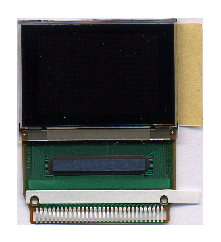
\includegraphics[height=3cm]{figures/displayandchip.eps}
 \caption{Sample of a commercial OLED device with integrated driver chip}
 \label{fig:displayandchip}
\end{figure}



A (passive matrix) OLED display has a matrix structure consisting of $n$ rows
and $m$ columns.  At any crossover between a row and a column there is
a vertical diode which works as a pixel. 
The image itself is given as an integral non-negative $n \times m$ matrix
$(r_{ij}) \in [0,\ldots,\varrho]^{n \times m}$ representing its RGB values.
Consider the contacts for the rows and columns as switches.  For the
time the switch of row $i$ and column $j$ is closed, an electrical
current flows through the diode of pixel $(i,j)$ and it shines. Hence,
we can control the intensity of a pixel by the two quantities
\emph{electrical current} and \emph{time}. 
The value $r_{ij}$ determines the amount of time within the time frame
in which the switches $i$~and~$j$ have to be simultaneously closed.
At a sufficient high frame rate e.g. 50 Hz, the perception by the eye
is the average value of the light emitted by the pixel and one sees the image.

The traditional addressing scheme is row-by-row. This means that the
switch for the first row is closed for a certain time while the
switches for the columns are closed for the necessary amount of time
dictated by the entries $r_{1j},\, j=1,\ldots,m$. Consequently the first
row can be displayed in time $\max \{ r_{1j}: j = 1, \ldots, m \}$.
Then the second row is displayed and so on. With this addressing
scheme, the pixels are idle most of the time and then have to shine
with very high intensity. This puts the diodes under stress and is a
major cause of the short lifetime of the displays. 


How can this lifetime problem be dealt with? The main idea is to save
time, or equivalently to lower the maximum intensity, by displaying
several rows at once. 

Consider the schematic image on the left of Fig.~\ref{fig:example}.
Let us compute the amount of time which is
necessary to display the image with this addressing scheme.  The
maximum value of the entries in the first row is $238$. This is the
amount of time which is necessary to display the first row. After that
the second row is displayed in time $237$. In total the time which is
required to display the image is $238+237+234+232+229=1170$ time
units.

\begin{figure}[ht]
  \centering
  $$
\columnseprule5mm
\xdefinecolor{r1}{RGB}{109,238,28}
\xdefinecolor{r2}{RGB}{112,237,28}
\xdefinecolor{r3}{RGB}{150,234,25}
\xdefinecolor{r4}{RGB}{189,232,22}
\xdefinecolor{r5}{RGB}{227,229,19}
\begin{matrix}
\rowcolor{r1} 109 & 238 & 28 \\
\rowcolor{r2} 112 & 237 & 28 \\
\rowcolor{r3} 150 & 234 & 25 \\
\rowcolor{r4} 189 & 232 & 22 \\
\rowcolor{r5} 227 & 229 & 19
\end{matrix}
\>\> = \>\>
\xdefinecolor{m1}{RGB}{0,82,25}
\xdefinecolor{m2}{RGB}{112,155,3}
\xdefinecolor{m3}{RGB}{0,41,22}
\xdefinecolor{m4}{RGB}{189,191,0}
\begin{matrix}
\rowcolor{m1}    \color{white}0 & \color{white} 82 & \color{white}25 \\
\rowcolor{m1}    \color{white}0 & \color{white} 82 & \color{white}25 \\
\rowcolor{m3}    \color{white}0 & \color{white} 41 & \color{white}22 \\
\rowcolor{m3}    \color{white}0 & \color{white} 41 & \color{white}22 \\
\rowcolor{black} \color{white}0 & \color{white}  0 & \color{white} 0 \\
\end{matrix}
\>\> + \>\> 
\begin{matrix}
\rowcolor{black} \color{white} 0 & \color{white}  0 & \color{white} 0 \\
\rowcolor{m2} \color{white} 112 & \color{white} 155 & \color{white} 3 \\
\rowcolor{m2} \color{white} 112 & \color{white} 155 & \color{white} 3 \\
\rowcolor{m4} \color{white} 189 & \color{white} 191 & \color{white} 0 \\
\rowcolor{m4} \color{white} 189 & \color{white} 191 & \color{white} 0
\end{matrix}
\>\> + \>\> 
\xdefinecolor{s1}{RGB}{109,156,3}
\xdefinecolor{s2}{RGB}{0,0,0}
\xdefinecolor{s3}{RGB}{38,38,0}
\xdefinecolor{s4}{RGB}{0,0,0}
\xdefinecolor{s5}{RGB}{38,38,19}
\begin{matrix}
\rowcolor{s1} \color{white} 109 & \color{white} 156 & \color{white}   3 \\
\rowcolor{s2} \color{white}   0 & \color{white}   0 &  \color{white}  0 \\
\rowcolor{s3} \color{white}  38 & \color{white}  38 &  \color{white}  0 \\
\rowcolor{s4} \color{white}   0 &  \color{white}  0 &  \color{white}  0 \\
\rowcolor{s5} \color{white}  38 & \color{white}  38 & \color{white}  19
\end{matrix}
$$
  \caption{An example decomposition}
  \label{fig:example}
\end{figure}

\noindent Now consider the decomposition of the image as the sum of the three
images on the right of Fig.~\ref{fig:example}. In the first image, each
odd row is equal to its even successor. This means that we can close
the switches for rows $1$ and $2$ simultaneously, and these two equal
rows are displayed in $82$ time units.  Rows $3$ and $4$ can also be
displayed simultaneously which shows that the first image on the right
can be displayed in $82+41$ time units. The second image on the right
can be displayed in $155+191$ time units while the third image has to
be displayed traditionally. In total all three images, and thus the
original image on the left via this decomposition, can be displayed in
$82+41+155+191+156+38+38=701$ time units. This means that we could
reduce the necessary time via this decomposition by roughly
$40\%$. We could equally display the image in the original $1170$ time
units but reduce the peak intensity, or equally the maximum electrical current
through a diode by roughly $40\%$.


We now show how to model the time-optimal decomposition of an image as
a linear program. 
To decompose $R$ we need to find matrices
$F^{(1)}=(f_{ij}^{(1)})$ and $F^{(2)}=(f_{ij}^{(2)})$ where $F^{(1)}$
represents the singleline part and $F^{(2)}$ the two doubleline parts.
More precisely, the $i$-th row of matrix $F^{(2)}$ represents the
doubleline covering rows $i$ and $i+1$.  Since the overlay (addition)
of the subframes must be equal to the original image to get a valid
decomposition of $R$, the matrices $F^{(1)}$ and $F^{(2)}$ must
fulfill the constraint $f^{(1)}_{ij} + f^{(2)}_{i-1,j} +
f^{(2)}_{ij}=r_{ij}$ for $i=1,\dots,n$ and $j=1,\dots,m$, where we now
and in the following use the convention to simply omit terms with
indices running out of bounds.  Since we cannot produce ``negative''
light we require also non-negativity of the variables
$f^{(\alpha)}_{ij}\geq0$.  The goal is to find an integral decomposition
that minimizes
\begin{equation*}
\sum_{i=1}^n \max \{ f^{(1)}_{ij}: 1 \leq j \leq m \} + \sum_{i=1}^{n-1} \max \{
f^{(2)}_{ij}: 1 \leq j \leq m \}\enspace.
\end{equation*}
This problem can be formulated as a  linear program by
replacing the objective by $\sum_{i=1}^n u^{(1)}_i +
\sum_{i=1}^{n-1}u^{(2)}_i$ and by adding the constraints $ f^{(\alpha)}_{ij} \leq
u^{(\alpha)}_i$.  This yields
\begin{align}
  \min~ & \sum_{i=1}^n u^{(1)}_i+\sum_{i=1}^{n-1}u^{(2)}_i\nonumber\\
  \text{s.t.}\quad & f^{(1)}_{ij} + f^{(2)}_{i-1,j} + f^{(2)}_{ij} = r_{ij}
  &&\text{for all $i,j$}\label{eqn:original}\\
  & f^{(\alpha)}_{ij} \leq u^{(\alpha)}_i
  &&\text{for all $i,j,\alpha$}\\
   & f^{(\alpha)}_{ij} \in\setR_{\geq 0}
  &&\text{for all $i,j,\alpha$} \nonumber\nonumber
\end{align}
%
Note that the objective does not contain the $f$-variables. By
decomposing images like this, the average lifetime of an OLED display
can be increased by roughly 100\%, see~\cite{EKX07}. 


\section*{Exercises}

\begin{enumerate}[1)]
\item A company produces and sells two different products.
Our goal is to determine the number of units of each product they should produce during one month,
assuming that there is an unlimited demand for the products,
but there are some constraints on production capacity and budget.

There are 20000 hours of machine time in the month.
Producing one unit takes 3 hours of machine time for the first product and 4 hours for the second product.
Material and other costs for producing one unit of the first product amount to 3CHF,
while producing one unit of the second product costs 2CHF.
The products are sold for 6CHF and 5CHF per unit, respectively.
The available budget for production is 4000CHF initially.
25\% of the income from selling the first product can be used immediately as additional budget for production,
and so can 28\% of the income from selling the second product.
\begin{enumerate}
\item Formulate a linear program to maximize the profit subject to the described constraints.
\item Solve the linear program graphically by drawing its set of feasible solutions and determining an optimal solution from the drawing.
\item Suppose the company could modernize their production line to get an additional 2000 machine hours for the cost of 400CHF.
  Would this investment pay off?
\end{enumerate}

\item Reformulate the following linear program in inequality standard form. 
The objective is to minimize
\begin{displaymath}
  -3 x_1 + 3 x_2 + 5 x_3 
\end{displaymath}
such that $x_1,x_2,x_3$ satisfy the constraints
\begin{equation}
  \label{eq:2}
  x_2+ 3 x_3 ≥ 4, 
\end{equation}
\begin{equation}
  \label{eq:3}
  2x_1 + 2  x_2 - 4 x_3  = -4, 
\end{equation}
as well as the lower bounds
\begin{equation}
  \label{eq:4}
  x_1≥0, x_2 ≥ 0, x_3 ≥ 0.
\end{equation}

  
\item A factory produces two different products.
To create one unit of product 1, it needs one unit of raw material $A$
and one unit of raw material $B$.
To create one unit of product 2, it needs one units of raw material $B$ and
two units of raw material $C$.
Raw material $B$ needs preprocessing before it can be used, which takes
one minute per unit. 
At most 20 hours of time is available per day for the preprocessing.
Raw materials of capacity at most 1200 can be delivered to the factory per day. 
One unit of raw material A, B and C has size 4, 3 and 2 respectively. 

At most 130 units of the first and 100 units of the second product can be sold
per day. The first product sells for 6 CHF per unit and the second one
for 9 CHF per unit.

Formulate the problem of maximizing turnover as a linear program in two variables and solve it.

\item Prove the following statement or give a counterexample:
The set of optimal solutions of a linear program is always finite.
\item Let (\ref{eq:lp-inequality}) be a linear program in inequality standard form, i.e.
\begin{equation} \label{eq:lp-inequality}
\max\{ c^T x \mid Ax \leq b, x \in \setR^n \}
\end{equation}
where $A \in \setR^{m \times n}$, $b\in \setR^m$, and $c\in\setR^n$.

Prove that there is an equivalent linear program (\ref{eq:lp-equality}) of the form
\begin{equation} \label{eq:lp-equality}
\max\{ \tilde c^T x \mid \tilde Ax = \tilde b, x \geq 0, x \in \setR^{\tilde n} \}
\end{equation}
where $\tilde A \in \setR^{\tilde m \times \tilde n}$, $\tilde b \in \setR^{\tilde m}$, and $\tilde c \in \setR^{\tilde n}$
are such that every feasible point of (\ref{eq:lp-inequality}) corresponds to a feasible point of (\ref{eq:lp-equality})
with the same objective function value and vice versa.

Linear programs of the form in (\ref{eq:lp-equality}) are said to be in \emph{equality standard form}.

\item  Model the linear program~\eqref{eqn:original} to decompose the EPFL logo with Zimpl. 
An incomplete model containing the encoding of the grayscale values of the logo can be found \href{http://disopt.epfl.ch/webdav/site/disopt/users/190205/public/logo\_dec.zmpl}{here}\footnote{http://disopt.epfl.ch/webdav/site/disopt/users/190205/public/logo\_dec.zmpl}.

Use an LP solver library of your choice to compute an optmal solution.

\end{enumerate}


% \bibliographystyle{abbrv}

% \bibliography{mybib,papers,books,my_publications}


%%% Local Variables: 
%%% mode: latex
%%% TeX-master: "lecture"
%%% End: 
